前章のように,日本では医療情報が全ての医療機関では共有されていない.
全ての医療機関で医療情報の共有を行おうとすると,
使用する電子カルテソフトの統一か,
規格の異なる出力ファイルの差を吸収して医療情報を扱うことの
どちらかが必要となる.
電子カルテソフトには多くの種類があり導入するソフトは
医療機関の診療科目に依存することがある.
つまり,使用する電子カルテソフトの統一は現実的ではない.
そこで,
患者が自身の医療情報を入力できて,
異なる形式からの入力に
対応した医療情報を共有するシステムを提案する.
提案システムの設計を図\ref{system_construct}の
UMLユースケース図と図\ref{class}のUMLクラス図によって示す.

\begin{figure}[htbp]
  \begin{center}
    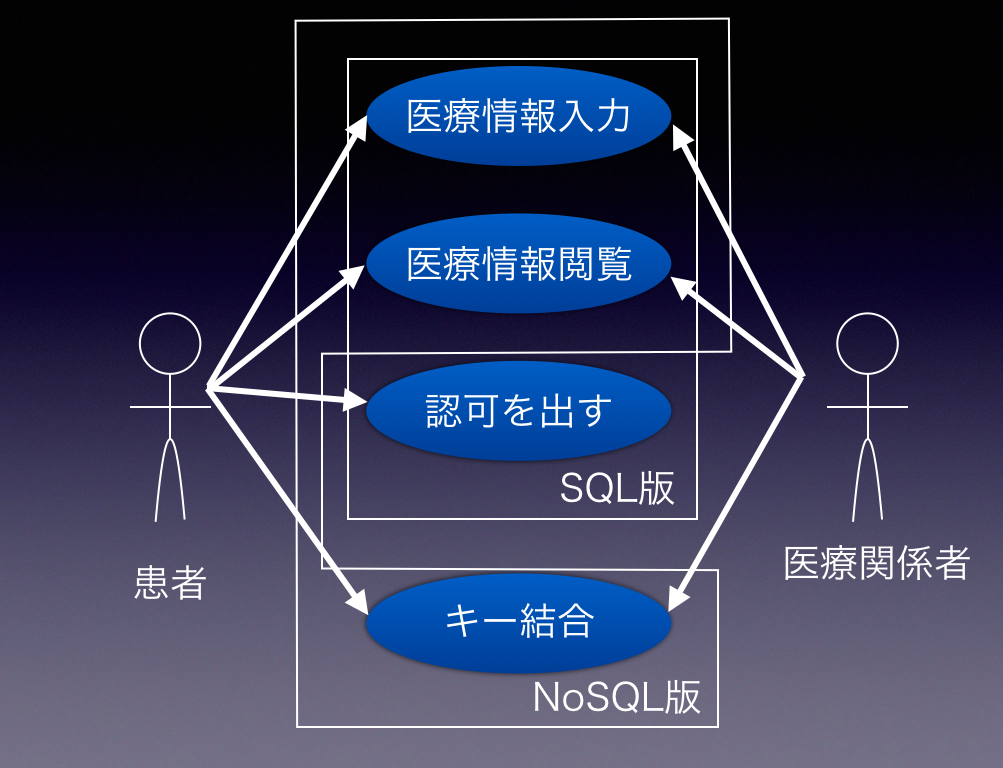
\includegraphics[width=10cm, bb=0 0 1003 768]{./gazou/system_construct2.png}
  \end{center}
  \caption{システムのUMLユースケース図}
  \label{system_construct}
\end{figure}

\begin{figure}[htbp]
  \begin{center}
    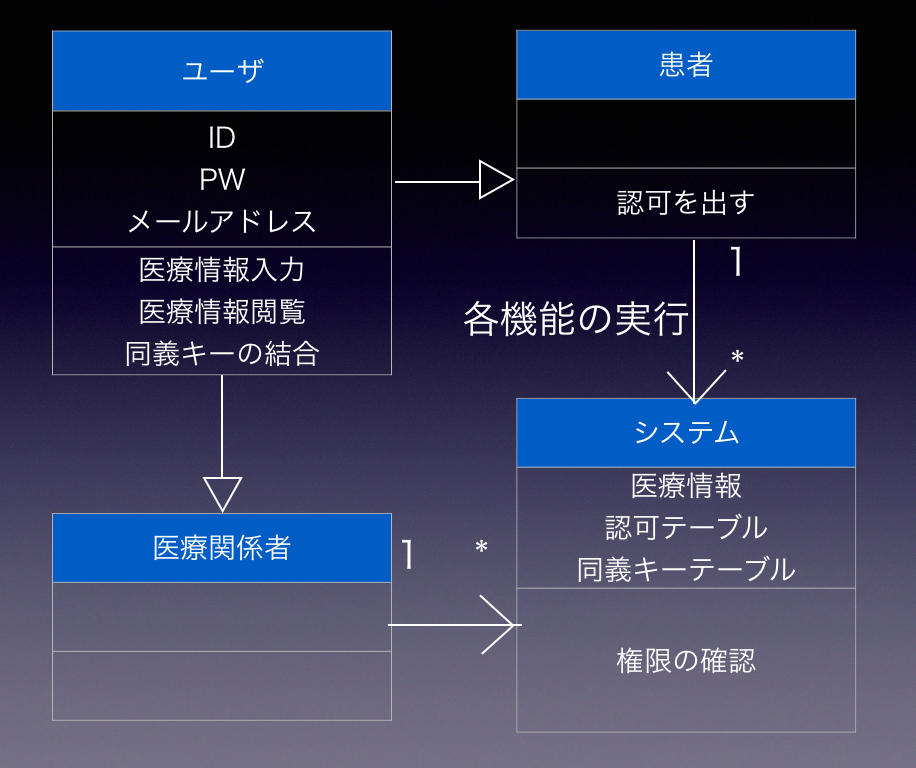
\includegraphics[width=10cm, bb=0 0 916 760]{./gazou/class.png}
  \end{center}
  \caption{UMLクラス図}
  \label{class}
\end{figure}

医療情報の入力と医療関係者に対する閲覧の機能は既存のシステムにも導入されていて,
医療情報共有システムとして必須と言える.

認可を出す機能は患者が利用できる機能で,
自身の医療情報を操作できる医療関係者を選択するためのものである.
現在は患者が医療情報を操作してよい医療関係者を選択する方式となっているが,
必要に応じて患者が操作されたくない医療関係者だけを指定する方式に切り替えることもできる.

キー結合とは
異なる形式の入力データは同じ意味の項目であっても,
厳密に同じ言葉を項目名にとっていないために生じる
問題を解決するための機能である.
例えば薬を処方した日という意味の項目に対して処方日という項目名と
日時という項目名をとっている場合がある.
ここでは便宜的に処方日と日時のように,
異なる項目名であるが同じ意味の項目の群を
同義キーと呼ぶ.
この同義キーを関連付ける機能を実装することで
異なる形式からの入力情報を関連付ける.
具体的な機能として,同義キーのうちのひとつが検索される際に,
その同義キーの群の項目も検索結果として反映させる.

これらの機能をユーザに提供することで,
患者が自身の医療情報を操作できて,
様々な形式の医療情報を入力として受け付ける
システムを開発する.
